\documentclass[12pt,usenames,dvipsnames]{beamer}

%\usetheme[progressbar=frametitle]{metropolis}
\usetheme[subsectionpage=progressbar]{metropolis}

\metroset{block=fill}
%\begin{itemize}[<+- | alert@+>]


\usepackage[utf8]{inputenc}
% Für Häkchen
\usepackage{ pifont }
\newcommand{\cmark}{\ding{51}}%
\newcommand{\xmark}{\ding{55}}%
% Farben
\usepackage{xcolor}

\usepackage{graphicx}
\graphicspath{ {images/} }

\setbeamertemplate{itemize item}{\tiny$\bullet$}
\setbeamertemplate{itemize subitem}{\tiny$\bullet$}

\title{PolyGlot-Database Performance}
\subtitle{Benchmark Framework - MongoDB vs Neo4J}
\author{Hyeon Ung Kim, Tim Niehoff}
%\institute{}
\date{6. August 2018}

\makeatletter
\setbeamertemplate{section page}{
  \centering
  \begin{minipage}{22em}
    \raggedright
    \usebeamercolor[fg]{section title}
    \usebeamerfont{section title}
    \centering\insertsectionhead\\[-1ex]
    \centering\usebeamertemplate*{progress bar in section page}
    \par
    \ifx\insertsubsectionhead\@empty\else%
      \usebeamercolor[fg]{subsection title}%
      \usebeamerfont{subsection title}%
      \centering\insertsubsectionhead
    \fi
  \end{minipage}
  \par
  \vspace{\baselineskip}
}
\makeatother

\begin{document}

	\maketitle
			
%	\begin{frame}{Gliederung}
%		\setbeamertemplate{section in toc}[sections numbered]
%\setbeamertemplate{subsection in toc}[subsections numbered]
%		\tableofcontents
%	\end{frame}
	\section{Aufgabenstellung}
	\begin{frame}{Heranführung}
	\begin{itemize}[<+- | alert@+>]
	\item Verschiedene DB Typen mit unterschiedlichen Vorteilen\footnote{ Inhalt der Folie von \url{https://dbs.uni-leipzig.de/file/Intro_bdprak_final.pdf}}
		\begin{itemize} [<+- | alert@+>]
	\item Relational: Sicherheit, homogene Daten
	\item Document: Flexibles Schema, Suchfunktionen
	\item Graph: Beziehungen, Traversal
	\end{itemize}
	\item Polyglot: Verwendung mehrerer DB-Typen für untersch. Anwendungsfälle
	\item Aufgabe: Vergleich einer
Graphdatenbank mit einer Dokumenten-Datenbank
	\end{itemize}	
	\end{frame}
		\begin{frame}{gegebene Werkzeuge}
		\begin{table}[]
\begin{tabular}{ll}

\includegraphics[width=0.2\textwidth]{java}  & 
\includegraphics[width=0.3\textwidth]{yelp} \\

\includegraphics[width=0.4\textwidth]{mongodb}  & 
\includegraphics[width=0.35\textwidth]{neo4j}
\end{tabular}
\end{table}
	\end{frame}
\begin{frame}<presentation:0>
\begin{itemize}
\item Mongo + Neo4j Driver
\item teilweise nicht ausgereift. Für das garantieren von beliebigen Queries muss geparst werden
\end{itemize}
\end{frame}
\section{Herausforderung: Gleicher Datensatz auf beiden DB}
\subsection{Mongo Connector + Neo4j Doc Manager}
\begin{frame}{Mongo Connector + Neo4j Doc Manager}
\begin{itemize}[<+- | alert@+>]
\item Software jeweils von MongoDB und Neo4j
\item Dauerhafte Synchronisation zwischen Mongo und Neo4j möglich
\item Generisches Erstellen des Neo4j Datenmodells 
\end{itemize}
\end{frame}
\subsection{Apoc}
\begin{frame}
\begin{itemize}[<+- | alert@+>]
\item Software von Neo4j zum Import von JSONs in Neo4j
\item keine automatische Synchronisierung zwischen Mongo und Neo4j
\item kein generisches Datenmodell
\item Vorteil des nutzerspezifischen Datenmodells: Ausnutzen graphdatenbankspezifischer Performanzvorteile
\end{itemize}

\end{frame}
\section{Resultat: PolyGDBP}
\subsection{Pipline und Workflow}
\begin{frame}
\begin{itemize}[<+- | alert@+>]
\item File Struktur (Main, Mongo, Neo4j, Benchmark)
\item Command line Interface
\item nur Queryangabe ist pflicht, alles andere optional.
\item gibt vorgefertigte Queries für Yelp Datensatz
\item Nutzer kann JSON Datensatz importieren
\item Wird in MongoCollections verarbeitet und durch MongoConnector erfolgt danach das Übertragen in Neo4j
\item Queries werden ausgeführt
\item vor und jedem dieser Schritte zeit gestoppt, geloggt und schließlich ausgegeben
\item kann mithilfe unserer Javascript Anwendung visualisiert werden.
\end{itemize}
\end{frame}
\section{Lets run it. With the help of YELP}
\subsection{Datensatz + DatenModell}
\begin{frame}
\begin{itemize}[<+- | alert@+>]
\item YELP = Suchmaschine und Empfehlungsportal für Restaurants und Geschäfte 
\item YELP Datensatz X GB groß
\item besteht aus X .jsons: users, business, review, ...
\item Beispiele eines JSON Business Objektes:
\item ...
\end{itemize}
\end{frame}
\begin{frame}{Neo4j Datenmodell}
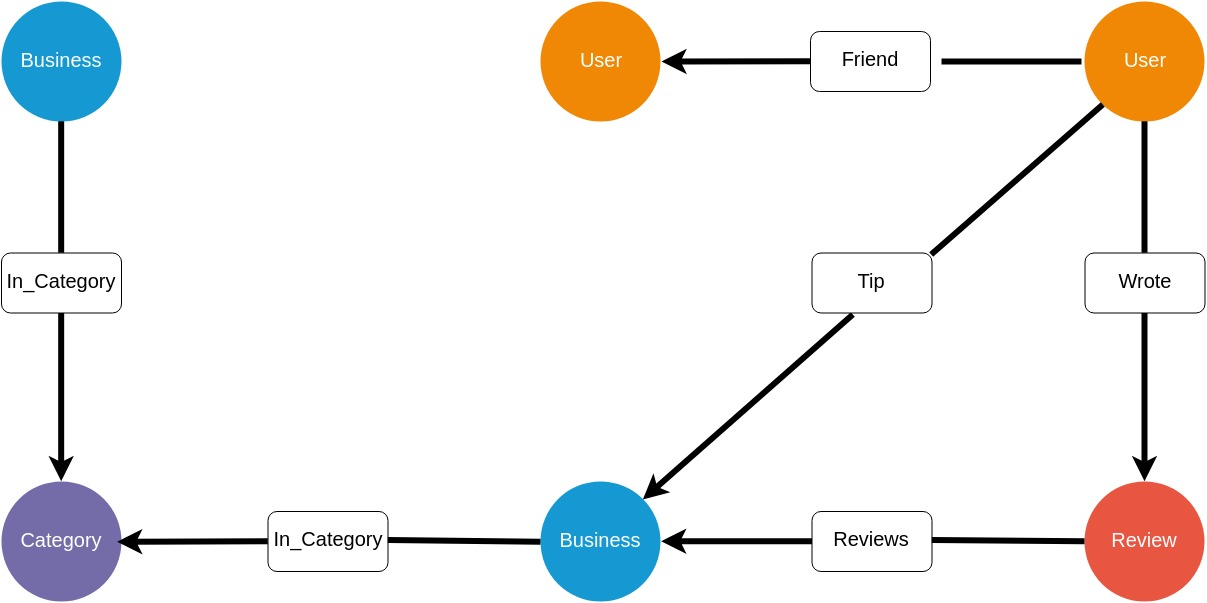
\includegraphics[width=1\textwidth]{neo4jModell}

\end{frame}
\subsection{Ergebnisse}
	\section{Zusammenfassung}
	\begin{frame}{Zusammenfassung}
	\begin{itemize}[<+- | alert@+>]
	\item Verschiedene DB-Typen haben versch. Vor- und Nachteile
	\item PolyG-DBP ist ein Framework zum Vergleich einer Dokument-DB mit einer Graphdatenbank
	\item konkret: MongoDB und Neo4j werden getestet
	\item Nutzer kann prebuilt queries ausführen lassen oder eigene Queries testen lassen
	\item Ausführungszeiten der Queries werden gemessen und verglichen
	\item Unsere Tests mithilfe von PolyG-DBP und Yelp zeigen: Neo4j und MongoDB siegen bei bestimmten Arten von Queries
	\end{itemize}
	\end{frame}
\begin{frame}[standout]
  Fragen und Diskussion
\end{frame}


\end{document}